\documentclass[preview]{standalone}
\usepackage{tikz}

\usetikzlibrary{shapes,decorations,arrows,calc,arrows.meta,fit,positioning}
\tikzset{
    -Latex,auto,node distance =1 cm and 1 cm,semithick,
    state/.style ={ellipse, draw, minimum width = 0.7 cm},
    point/.style = {circle, draw, inner 						sep=0.04cm,fill,node contents={}},
    bidirected/.style={Latex-Latex,dashed},
    el/.style = {inner sep=2pt, align=left, sloped}
}
\begin{document}

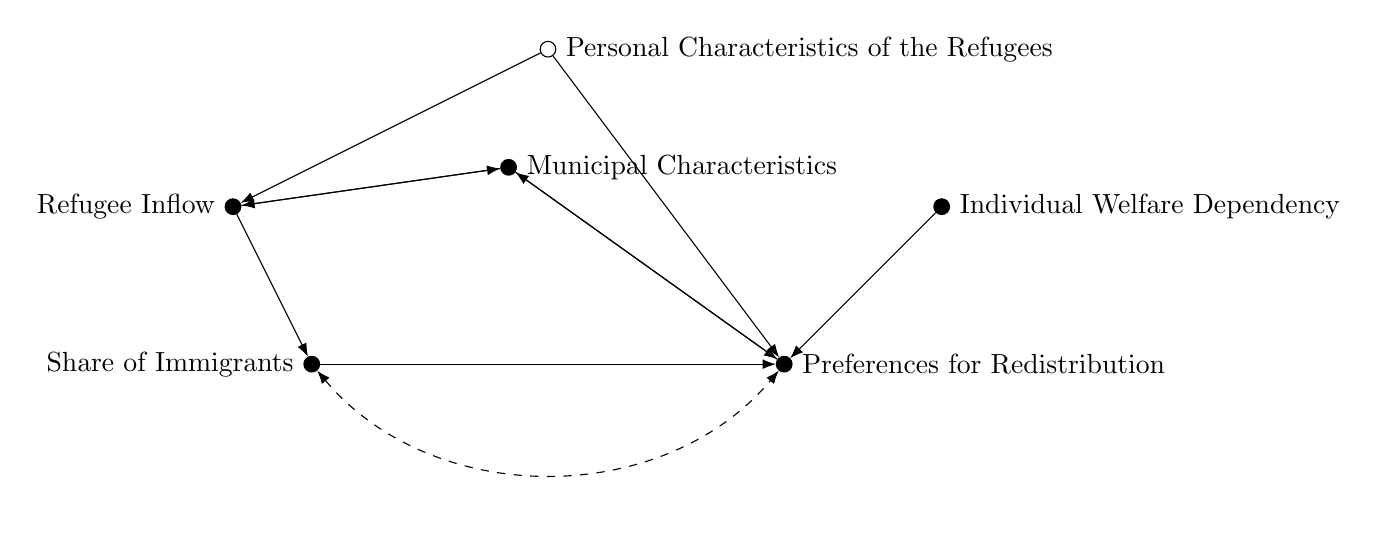
\begin{tikzpicture}
	\tikzstyle{o}=[circle, draw, inner sep = 2, fill = 				black]
	\tikzstyle{u}=[circle, draw, inner sep = 2]
	
	\node[o, label = left: Share of Immigrants] (1) at 				(0,0){};
    \node (2) [o, label = right: Preferences for 					Redistribution] at (6,0){};
	\node (3) [o, label = left: Refugee Inflow ] at (-1,2)			{};
	\node (4) [o, label = right: Municipal 							Characteristics] at (2.5,2.5){};
	\node (5) [o, label = right: Individual 						Welfare Dependency] at (8,2){};
	\node (6) [u, label = right: Personal Characteristics 			of the Refugees] at (3,4){};

    \path (1) edge  (2);
    \path[bidirected] (1) edge[bend right=50]  (2);
    \path (3) edge (1);
    \path (4) edge (3);
    \path (3) edge (4);
    \path (4) edge (2);
    \path (2) edge (4);
    \path (5) edge (2);
    \path (6) edge (3);
    \path (6) edge (2);
\end{tikzpicture}
\end{document}